\documentclass[MTRX3700report.tex]{subfiles}
%\documentclass{article}
%\usepackage{graphicx}
%\usepackage{float}
%\usepackage{listings}

\begin{document}

%\section{Software Design}  dont include at the end but you can for seperate builds
%The software requirements and overview have been dealt with elsewhere in this document. The present section addresses the design and implementation of the software that forms the X system.
\subsection{Software Design Process}
%How you went about designing the software – top down, bottom up, OOD, functional view, etc.
The software was designed in a modular top down manner for both the robot and the controller. All code for the robot and controller where designed tested and implemented independent of each other with the exception of the Serial Communications module which was identical on both sides. Furthermore each module designed to operate as independently as possible from the others for easier integration.
\subsubsection{Software Development Environment}
%The tools that were used, both software (compilers, assemblers, etc) and hardware (development boards, etc.).
All software was created and compiled using MPLAB X IDE v3.
Software was then run and debugged using  the ICD 3 first on the PIC18F452 development board and then on the PIC18F4520 minimal board.
\subsubsection{Software Implementation Stages and Test Plans}
%Describe the way you went about implementing the software - staged implementation, pseudocode (PDL), unit testing procedures, integration testing, etc. Identify dependencies – e.g this had to be done before that, etc.
Each software was first implemented, debugged and tested on the PIC18F452 development board until it worked.

The modules where then implemented on the PIC18F4520 minimal board and integrated in the following order:
	\begin{enumerate}
		\item \textbf{LCD and Menu Nav} on the Controller.
		\item \textbf{The buttons and Joystick} was integrated with the Menu Nav of the controller.
		\item \textbf{PWM motors} operation and control on the jousting robot.
		\item \textbf{Serial Communications} was then integrated to both the controller and jousting robot and tested. Once this was working the Controller was fully integrated.
		\item \textbf{Manual Mode} was then integrated on to the robot and tested with the controller via Serial Communications. 
		\item \textbf{IR Sensors} was then integrated to the robot along with Full Auto and Assited mode.
		\item After this was all integrated further tests and where conducted for operation under Manual, User Assist and Auto modes for the jousting robot using the joystick and button controller inputs.	
	\end{enumerate}

\subsection{Software Quality Assurance}
%Describe any measures that were taken to control (improve) the software quality – code or documentation standards, code walkthroughs, testing and validation, etc.
Each module had its own .c file and its own header file. All interactions between different modules were outlined in each header file.
A code header block was used for each file indicating the following in order:

	\begin{itemize}
		\item The module this file applies to.
		\item Date created and by whom.
		\item Date Last edited by whom and details of edit.
		\item File Description
		\item File Dependencies
		\item Current issues with file
	\end{itemize}
	
Another method used to ensure the quality of software was to implement all interrupts in the same file Interrupt\textunderscore Definition\textunderscore Robot calling functions from the respective modules. 

\subsection{Software Design Description}
\subsubsection{Architecture}
%Describe the high-level architecture of the software – that is, the top-level flow of control, and how the various functional modules communicate.\\
%In this section, you can put state transition diagrams, sequence diagrams, etc.

The following state transition diagrams show how the run modes are changed both for the controller and robot. Once a change is made on the controller the same change is made on the robot. Refer to Serial communications module for more information on how these changes occur. 
	\begin{figure}[h]
		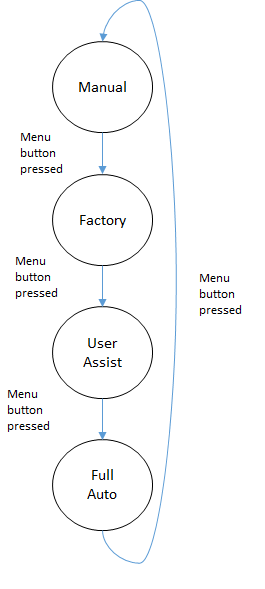
\includegraphics[scale=0.5]{controller_std.png}
		\centering
		\caption{Controller State Transition Diagram}
	\end{figure}
	
	\begin{figure}[h]
		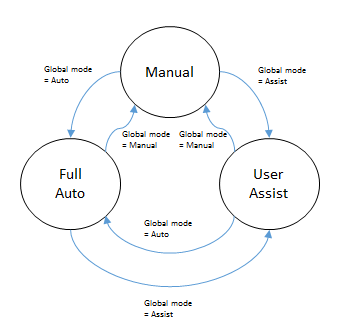
\includegraphics[scale=0.7]{robot_std.png}
		\centering
		\caption{Robot State Transition Diagram}
	\end{figure}

\subsubsection{Software Interface}
%Describe the public interface of each software module.
The User only has control over the mains for both the commander and the robot.
The main for the commander consists of the menu navigation and all interaction with user is displayed on the LCD. For the robot the main contains the different modes during runtime: Manual, Assisted and Auto. The user can choose which mode and run it through the commander and in the case of manual use the joystick to control the motion of the jousting robot.


\subsubsection{Software Components}
%This is a detailed view of the internal workings of each of the software modules.

Commander:
\begin{itemize}
	\item Menu Navigation.
	\item Menu Navigation submodule LCD.
	\item Serial Communications. 
	\item Analog to Digital conversion.
\end{itemize}
	
Jousting Robot:

\begin{itemize}
	\item Manual Mode
	\item Assist Mode
	\item Full Auto Mode
	\item PWM motors.
	\item IR Sensors.
	\item Serial Communications.
	\item Analog to Digital Conversion.
\end{itemize}

\subsection{Preconditions for Software}
\subsubsection{Preconditions for System Startup}
%Describe any preconditions that must be satisfied before the system can be started.
Either system Robot or Controller can startup in any order and both can operate. However any changes made on the controller (ie. changing global variables, mode or pressing run button) will not have any effect on the robot unless made while the robot has started up and operational.
\subsubsection{Preconditions for System Shutdown}
%Describe any preconditions that must be satisfied before the system can be stopped.
Precautions have not been taken to stop the robot when the controller is in operation. This means the robot will continue to operate as it was last instructed if the controller suddenly shuts down. However once the controller is restarted normal operation is resumed. 


\end{document}